% Définition du répertoire contenant les images
\graphicspath{{IMAGE/}}

% FRAME Intro
\begin{frame}


\includegraphics[width=12cm]{Logos.pdf}

\vfill

\begin{center}

\vspace*{1.5cm}

\LARGE
\textbf{Interactions}

\vspace*{1.5cm}
 DELHI GIS-R School


\large
9-12\up{th} April 2019

\vspace*{1.5cm}


\textbf{Hadrien Commenges \& Paul Chapron}

{\small

\vspace*{0.1cm}

\url{hadrien.commenges@univ-paris1.fr}

\url{paul.chapron@ign.fr}
}

\end{center}

\end{frame}



% FRAME
\begin{frame}{Use case}

\begin{block}{Interaction}
Relationship among objects.  An interaction may be unidirectional, bi-directional or multi-directional . 
If the entities are spatial objects, interaction always integrate a spatial dimension.
\end{block}

~

Relationships come in many forms

\begin{itemize}
\item Environment: migratory birds, climate refugees, home-to-work commutes, etc.
\item «Material realm»: commercial exchanges, percolation,   
\item «Immaterial realm» : twin-towns, Facebook friendship, co-authorship, etc.
\end{itemize}


~

\textbf{What kind of geographical information is concerned ?}



$\rightarrow$ \textit{TYPE 1 - Geographical Objects}

$\rightarrow$ \textit{TYPE 2 - Occurrences}



\end{frame}



% FRAME
\begin{frame}{Relations Modeling}

Interacting systems can be represented  by the \textbf{relations} between constitutive \textbf{entities} , either as an \textbf{(adjacency) matrix} or as a \textbf{list of links}, weighted or not. (cf Graphs)

%TODO figure EN 
\begin{figure}
  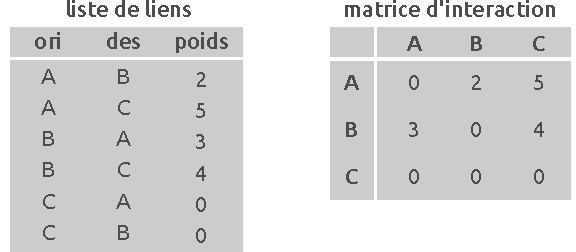
\includegraphics[width=9cm]{MatriceOD.pdf}
\end{figure}

\end{frame}



% FRAME
\begin{frame}{Distance and Interaction}

Spatial interactions imply \textbf{distance}.

~

\begin{itemize}
  \item Spatial interaction considers \textbf{ travel as an effort }.
  \item Spatial interaction confront \textbf{connecting entities} and the \textbf{distance induced decay}.
  \item Spatial interaction comes in two flavors : \textbf{relationships between locations}  or \textbf{attraction/influence of a location on the others}. 
  \begin{itemize}
  \item The first relies on \textbf{flow analysis}
  \item The second relies on \textbf{position analysis}(\textit{ Accessibility})
  \end{itemize}
\end{itemize}

\end{frame}


% FRAME
\begin{frame}{What is distance ?}


\textbf{In Geography}, distance is a separation, requiring \textbf{effort} to be crossed. Distance is a \textbf{friction}, a barrier:

\begin{itemize}
  \item \emph{«Everything is related to everything else, but near things are more related than distant things»} (Tobler)
\end{itemize}

~ 

\textbf{In Maths}, a distance is a function satisfying the following conditions 

\begin{itemize}
  \item Symmetry $d(a, b) = d(b,a)$
  \item Identity of indicernibles : $d(a, b) = 0 \Longleftrightarrow a = b$
  \item Triangle inequality: $d(a,c) \leq d(a,b) + d(b,c)$
\end{itemize}

\end{frame}


% FRAME
\begin{frame}{Euclidean Distance }


\textbf{For a n-dimensional vector:}

\begin{equation}
  \nonumber
  d(a,b) = \sqrt{\sum_{i=1}^n (a_i - b_i)^2}
\end{equation}

\end{frame}


% FRAME
\begin{frame}{Manhattan Distance}

\textbf{2D vector : }

\begin{figure}
  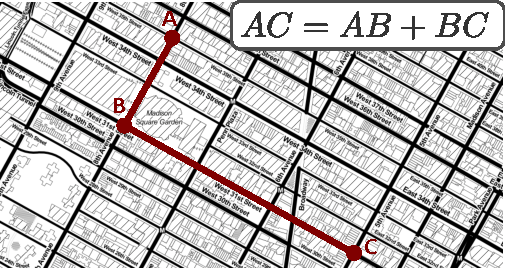
\includegraphics[width=8cm]{DistancesMan.pdf}
\end{figure}

\textbf{For a n-dimensional vector:}

\begin{equation}
  \nonumber
  d(a,b) = \sum_{i=1}^n |a_i - b_i|
\end{equation}

\end{frame}






% FRAME
\begin{frame}{Flow modeling}

\textbf{Original gravity model:}

\begin{equation}
\nonumber
T_{ij} = k \frac{P_i P_j}{D_{ij}^{2}}
\end{equation}

~
With $T_{ij}$, the flow from location $i$ to $j$.

$k$ a constant

$P_i$ the mass of location $i$

$D_{ij}$ the distance between location $i$ and $j$.


~

Many variations exist according to the choice of the terms:

\begin{itemize}
  \item \textbf{Masses:} populations, jobs , emissions, attractions
  \item \textbf{Masses weights:} multiplying factors or exponents
  \item \textbf{Friction function (distance):} negative powers, negative exponent
  \item \textbf{Margin Constraints:} double, simple, none
  \item \textbf{Numeric Resolution } 
\end{itemize}


\end{frame}


% FRAME
\begin{frame}{Modélisation des flux: formalisation}

\textbf{Le modèle d'opportunités interposées} (Stouffer 1960) s'écrit:

\begin{equation}
\nonumber
T_{ij} = k_i O_i \left[\exp(-\alpha x_{j-1}) - \exp(-\alpha x_{j}) \right]
\end{equation}

~

\textbf{Le modèle de radiation} (Simini \textit{et al.} 2012) s'écrit:  

\begin{figure}
  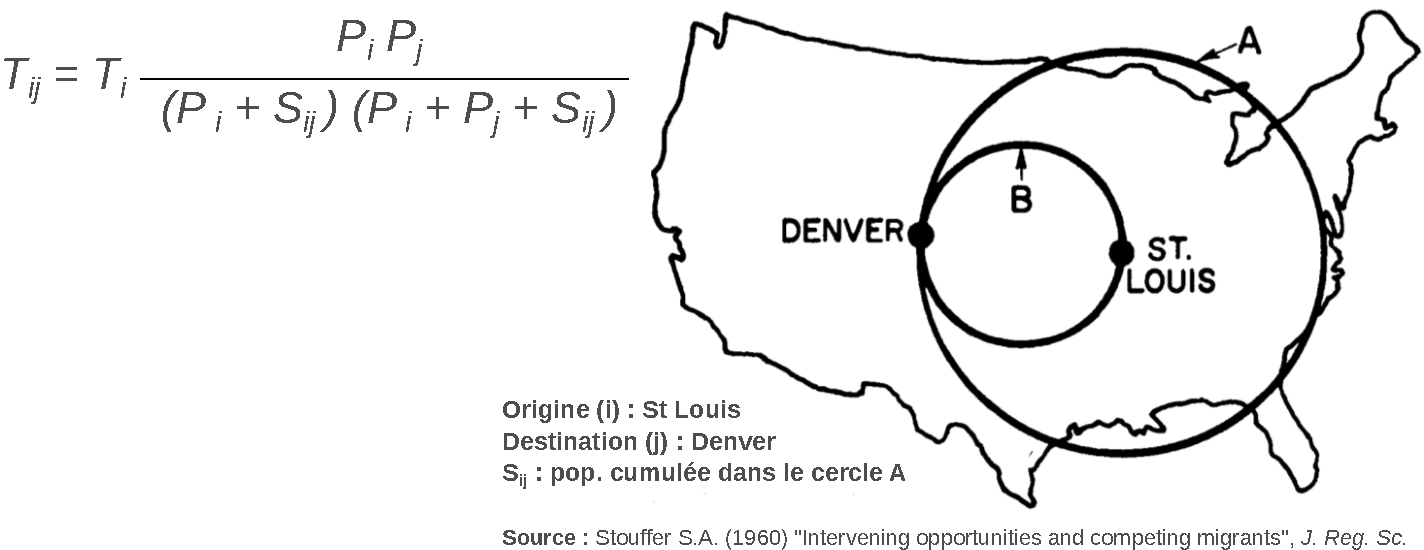
\includegraphics[width = 110mm]{CercleStouffer.pdf}
\end{figure}

\end{frame}


% FRAME
\begin{frame}{Network Analysis}

Leonhard Euler and the \textbf{Seven Bridges of Königsberg} (Kaliningrad).


\begin{figure}
  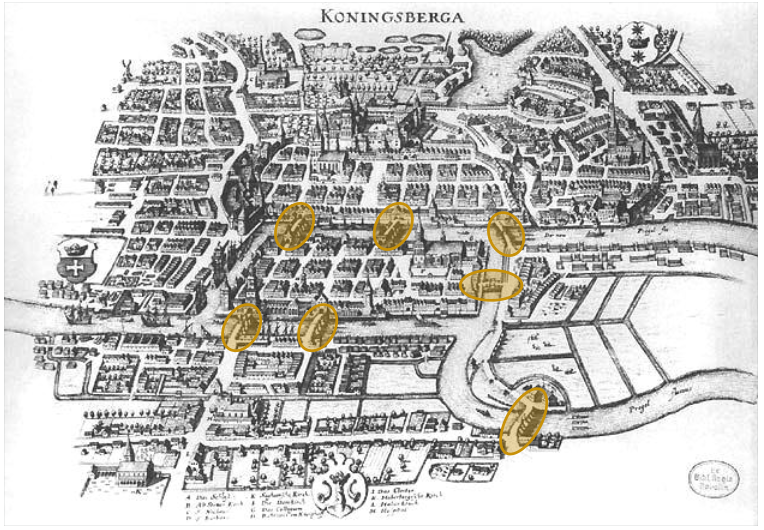
\includegraphics[width=10cm]{Konigsberg.png}
\end{figure}

\end{frame}


% FRAME
\begin{frame}{Network analysis}

\begin{figure}
  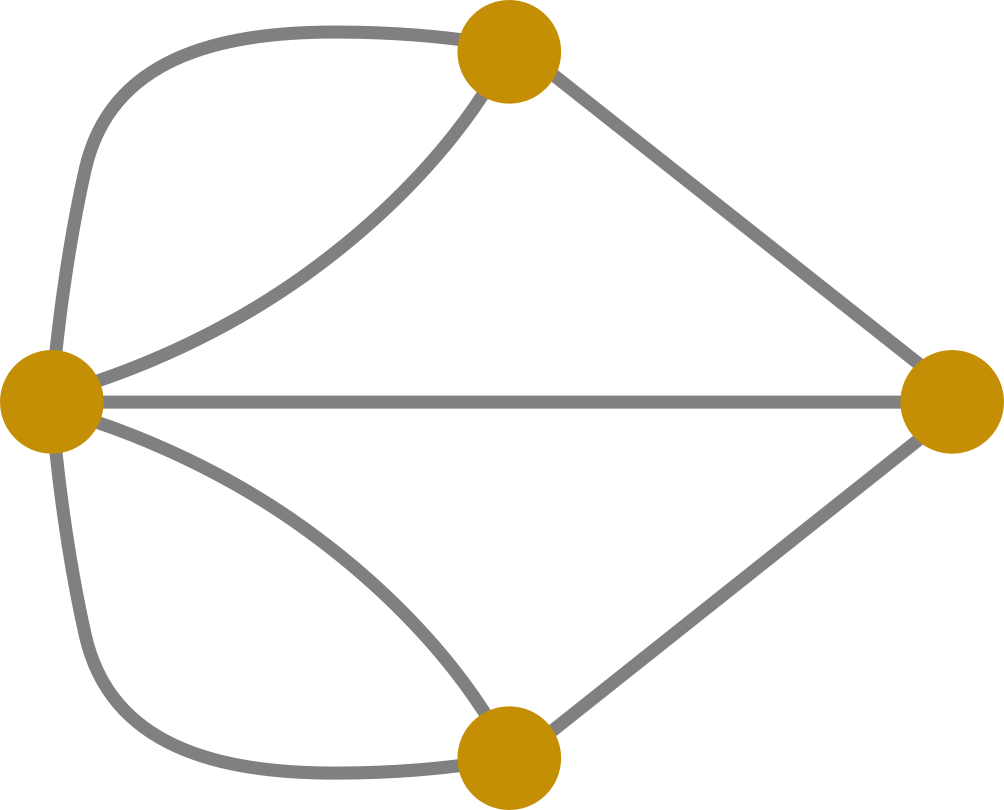
\includegraphics[width=5cm]{Konigsberg_graph.png}
\end{figure}

~

\begin{itemize}
\item No \textbf{cycle eulérien} (parité des liens incidents)
\item Pas de \textbf{chaîne eulérienne} (continuité du tracé)
\end{itemize}


\end{frame}



% FRAME
\begin{frame}{Graphs}

A graph is a set of \textit{vertices}) connected by \textbf{edges}.



Examples:

\begin{itemize} 
  \item \textbf{Transportation networks  :} e.g. Subway: nodes are  stations,  edges are lines.
  \item \textbf{Social networks:} individuals (nodes) , social interactions (edges)
  \item \textbf{Scientific collaboration networks:} Co-autorship (edges) among researchers (nodes)
  \item \ldots
\end{itemize}

\end{frame}




% FRAME
\begin{frame}{Types of graphs}

\textbf{Undirected graph:}

\begin{figure}
  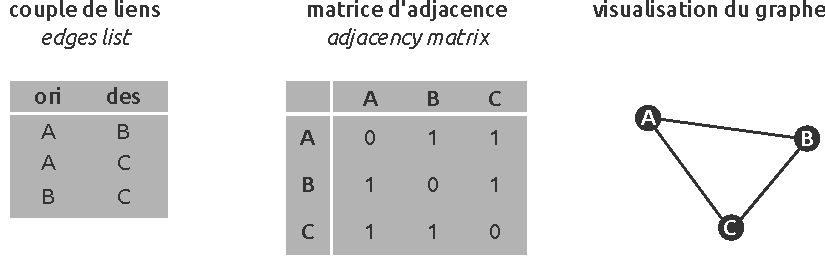
\includegraphics[width=12cm]{MatGraph3.pdf}
\end{figure}

\end{frame}


% FRAME
\begin{frame}{Types of graphs}

\textbf{Directed graph :}

\textit{arcs} are employed instead of \textit{edges} who are "undirected".

%TODO image EN
\begin{figure}
  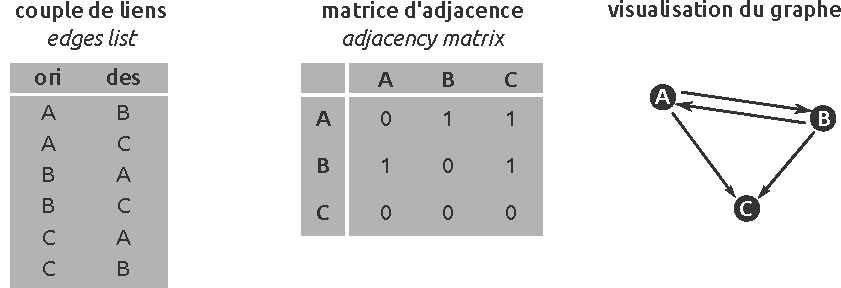
\includegraphics[width=12cm]{MatGraph2.pdf}
\end{figure}

\end{frame}



% FRAME
\begin{frame}{Types of graphs}

\textbf{Weighted directed graph:}

%TODO image EN
\begin{figure}
  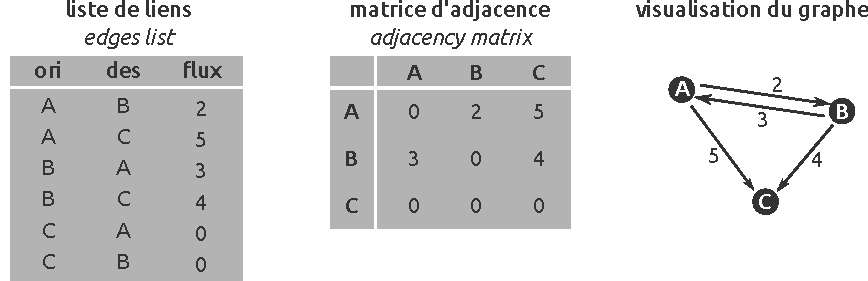
\includegraphics[width=12cm]{MatGraph1.pdf}
\end{figure}

Also :
\begin{itemize}
  \item Weighted undirected graphs
  \item Multi-graph ()
  \item Multi-partite graphs (several types of nodes )
  \item Hypergraphs (links between more than 2 nodes)
  \item \ldots
\end{itemize}

\end{frame}





% FRAME
\begin{frame}{Network analysis : measures}

\textbf{Global measures:}

\begin{itemize}
\item number of nodes
\item number of edges
\item connected components
\item Density (ratio nodes)
\item Diameter : length of the longest shortest paths 
\item Connectivity : number of edges and possible number of edges
\end{itemize}

~

$\rightarrow$ \textbf{Nombre maximum d’arcs (sans boucle):}

\begin{itemize}
\item pour un graphe planaire: $3V - 6$
\item pour un graphe non planaire non orienté: $\frac{V(V-1)}{2}$ 
\item pour un graphe non planaire orienté: $V(V-1)$
\end{itemize}

\end{frame}

% FRAME
\begin{frame}{Principales mesures descriptives}

\textbf{Mesures locales de centralité:}

\begin{itemize}
\item Degré: nombre d'arcs incidents (nbr. de voisins)
\item Degré pondéré: nbr. d’arcs incidents pondérés
\item Centralité de proximité (\textit{closeness}): inverse de la somme des distances à tous les autres noeuds
\item Centralité d'intermédiarité (\textit{betweenness}): nombre de plus courts chemins passant par un noeud (standardisé)
\end{itemize}


\end{frame}
